%
% File summer.tex
%
% Contact: koller@ling.uni-potsdam.de, yusuke@nii.ac.jp
%%
%% Based on the style files for ACL-2013, which were, in turn,
%% Based on the style files for ACL-2012, which were, in turn,
%% based on the style files for ACL-2011, which were, in turn, 
%% based on the style files for ACL-2010, which were, in turn, 
%% based on the style files for ACL-IJCNLP-2009, which were, in turn,
%% based on the style files for EACL-2009 and IJCNLP-2008...

%% Based on the style files for EACL 2006 by 
%%e.agirre@ehu.es or Sergi.Balari@uab.es
%% and that of ACL 08 by Joakim Nivre and Noah Smith

\documentclass[11pt]{article}

\usepackage{acl2014}

\usepackage{times}
\usepackage{url}
\usepackage{latexsym}
\usepackage{color}
\usepackage{amssymb}
\usepackage{amsmath}
\usepackage{graphicx}

\DeclareMathOperator*{\argmax}{arg\,max}

\title{Summer Research Paper}

\author{Will Povell \\
  Baltimore Polytechnic Institute \\
  {\tt willipovell@gmail.com} \\\And
  Matt Post \\
  Johns Hopkins University \\
  {\tt post@cs.jhu.edu} \\\And
  Frank Ferraro \\
  Johns Hopkins University \\
  {\tt ferraro@cs.jhu.edu}}

\date{}

\begin{document}
\maketitle

\begin{abstract}
  A review of basic knowledge about the field of computation linguistics and a description of what I've accomplished over the summer.
\end{abstract}

\section{Introduction}

The field of computational linguistics concerns using computer science, machine learning, statistics and other related fields to analyze and model language. This can be used to solve many problems, from detecting spam to improving human-computer interaction.

\subsection{Natural Language Processing}

\subsubsection{N-grams}

N-grams are a very commonly used tool in computational linguistics for modeling language. N-grams work by assigning a sequence of tokens (words, punctuation, etc.) of length $N$ a probability of occurring. This probability is equal to
$$ P\left(w_i | w_{1:i-1}\right) = \frac{u\left(w_{1:i-1}, w_i\right)}{\sum\limits_{v \in V} u\left(w_{1:i-1}, v\right)} $$
where $u$ is an unnormalized probability function that meets the following conditions
\begin{gather*}
u \geq 0, \\
\sum\limits_{v \in V} u\left(w_{1:i-1}, v\right) > 0
\end{gather*}

Here, $w$ represents a token and the notation $w_{1:i-1}$ is equivalent to the sequence of tokens $w_1, w_2, \cdots, w_{i-1}$. Additionally, $V$ represents the vocabulary set, with the sum iterating over each type $v$.

If you let
$$ u\left(w_{i-1}, w_i\right) = c\left(w_{i-1}, w_i\right) $$
\quad then
\begin{align*}
P\left(w_i \vert w_{i-1} \right) &= \frac{ c\left( w_{i-1}, w_i \right) }{ \sum\limits_{v \in V} c\left( w_{i-1}, v \right)} \\
&= \frac{ c\left( w_{i-1}, w_i \right) }{c\left( w_{i-1} \right) }
\end{align*}

where $c \left( w_1, w_2, \cdots, w_i \right)$ returns the number of times the sequence $w_1, w_2, \cdots, w_i$ occurred in the training data.

The particular N-gram example used is called a bigram because it looks at token sequences of length two. If it is a single token it is an unigram, three tokens it is a trigram, four tokens is a 4-gram, and so on.

$\sum\limits_{v \in V} c\left( w_{i-1}, v \right) = c\left( w_{i-1}\right)$ due to the fact that every time a two token sequence occurs, that first token in the sequence also occurs. Therefore, the sum of all the two token counts is equal to the one token count, called the marginal count. In a more general form,

$$ c\left(w_1, w_2, \cdots, w_i\right) =  \sum\limits_{v \in V} c\left(w_1, w_2, \cdots, w_i, v\right) $$

An example use of an N-gram model would be when you want to predict the next word in a sequence. If I have the sequence "How are", you could use an N-gram trained on other data to try and predict the next word by iterating over your vocabulary and choosing the highest probability $\argmax\limits_{w \in V} P\left( w \; \vert \; \text{How}, \text{are} \right)$. This could, for example, be "you" where $P\left( \text{you} \; \vert \; \text{How}, \text{are} \right) = 0.7$. In this example, the N-gram is a trigram (3-gram) as it uses 3 tokens in calculating the probability.

\subsubsection{Evaluation}

\paragraph{Normalized Log-Likelihood}

Minuscule probabilities are difficult to deal with due to limits on the number of significant digits in floating point point arithmetic. A way to solve this is to get the log of the probabilities. From there, a multiplication of probabilities becomes an addition of the log-probabilities.

This can be used by N-gram models as a way to gauge similarity between text. If you train an N-gram model on a dataset and then "score" another dataset by adding the log-probabilities of every N-gram in the scoring dataset, you get the log-likelihood. The more negative the likelihood is, the more "surprised" your model is by the text. The log-likelihood can be calculated as follows for the bigram

$$ \mathcal{L}\left(\mathcal{H}\right) = \sum\limits_{v, w \in V} N\left(v, w \right) \log P\left(w \vert v \right) $$

This value can be normalized to make comparisons easier, as follows

$$ \mathcal{L}_\mathcal{N}\left(\mathcal{H}\right) = \frac{ \mathcal{L}\left(\mathcal{H}\right) }{T} $$

where $T$ is the number of tokens in the held-out data.

An example usage of this would be to train a model on email spam, and then calculate the log-likelihood of another email. The closer the email's log-likelihood is to zero, the more likely that it is spam.

\paragraph{Maximization}

When tuning the amount of smoothing for a model, we often want to maximize the log-likelihood on a held-out dataset. This can be done using the derivative of the log-likelihood and gradient descent.

The derivative of an additively smoothed bigram log-likelihood can be derived as follows

\begin{align}
P\left(\mathcal{H}\right) &= \sum\limits_{v, w \in V} N\left(v, w\right) \log P^*\left(w \vert v\right) \\
&= \sum\limits_{v, w \in V} N\left(v, w\right) \log \frac{c\left(v, w\right) + \alpha}{c\left(v\right) + V\alpha} \\
&= \sum\limits_{v, w \in V} N\left(v, w\right) \log\left(c\left(v, w\right) + \alpha\right) - \log\left( c\left(v\right) + V\alpha \right)
\end{align}

$$ P^\prime\left(\mathcal{H}\right) = \sum\limits_{v, w \in V} N\left(v, w\right) \left(\frac{1}{c\left(v, w\right) + \alpha} - \frac{V}{c\left(v\right) + V\alpha }\right) $$

From there, log-likelihood can be maximized using gradient descent, described as follows, letting $f = P$ with $x$ representing the amount of smoothing (setting $x$ to an arbitrary start value).

\begin{gather*}
d = \text{precision} \\
\epsilon = \text{step size} \\
\mathcal{G}\left(x, f \right) =
\begin{cases}
\mathcal{G}\left(x + \epsilon \cdot f^\prime\left(x\right), f \right) & \text{if } \vert x - \epsilon \cdot f^\prime\left(x\right) \vert > d \\
x & \text{else}
\end{cases}
\end{gather*}


\subsubsection{Smoothing}

Simple N-gram models work as described above, but they can be greatly improved. Higher-order models especially suffer from over-fitting where they become too specialized to the dataset they were trained on, generalizing poorly. Data is often very sparse with many singletons (types that only occur once) and very few words that occur many times.

This problem of data sparsity can be seen in the following graph

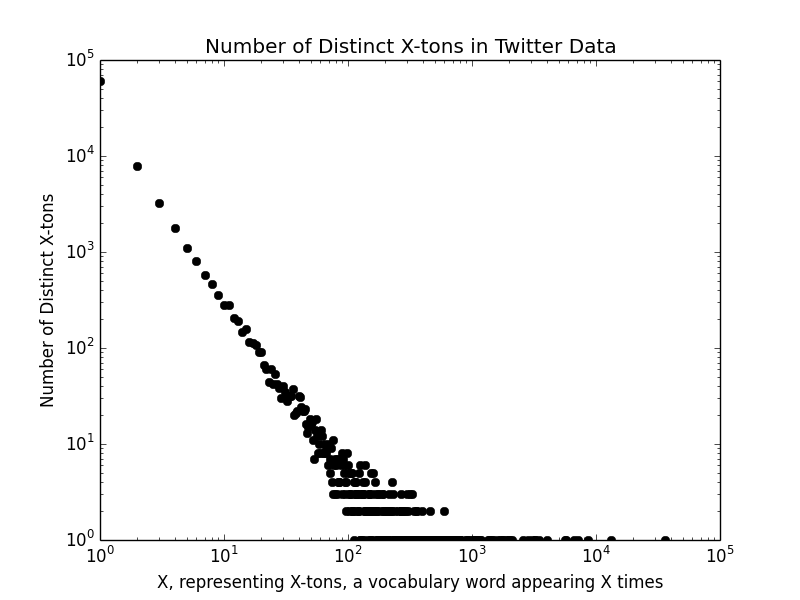
\includegraphics[width=218px]{graphs/x-ton.png}

Note that both scales are log-scales and that the relationship in negatively exponential.

Smoothing the N-gram probability distribution can help alleviate this problem by moving probability mass to lessen extremes and prevent counts that are equal to 0.

\paragraph{Additive}

One method of smoothing is called additive smoothing. This method works by adding a certain amount $\alpha$ to every count. Using this type of smoothing, the probability function is calculated as follows

$$ P^*\left(w_i \vert w_1, w_2, \cdots, w_{i-1} \right) = \frac{ c\left( w_1, w_2, \cdots, w_i \right) + \alpha}{ c\left( w_1, w_2, \cdots, w_{i-1} \right) + V\alpha } $$

where $V$ is the length of the vocabulary.

\paragraph{Other Interpolations}

An interesting thing to note about additive smoothing is that it is also just a linear interpolation between a bigram probability distribution and uniform probability distribution and can also be represented (for a bigram model) as follows

$$ P^*\left( w \vert v \right) = \lambda \frac{c\left( v, w \right)}{c\left( v\right)} + \left( 1 - \lambda \right) \frac{1}{V} $$

where $0 < \lambda < 1$. For the full derivation of this, see Appendix A.

Other interpolations can also be used. For example, you can interpolate bigram, unigram, and uniform models as follows

\begin{gather*}
P\left( w \vert v \right) = \lambda \frac{c \left(v, w\right)}{c \left(v\right)} + \mu \frac{c \left(v\right)}{N} + \theta \frac{1}{V} \\
\text{where} \\
\lambda + \mu + \theta = 1 \\
0 \leq \lambda, \mu, \theta \leq 1
\end{gather*}

The values for $\lambda$, $\mu$, and $\theta$ can be varied to maximize the generalization of the model.

The reason that interpolation is useful is it averages multiple models that are all able to partially explain the generative story of the text.

For example, say there are two probability distributions, $\mathcal{F} = N\left(-3, 1\right)$ and $\mathcal{G} = N\left(3, 1 \right)$, both normal distributions but with different means. There is also a weighted coin that has a $0.3$ chance of landing heads up (Bernoulli(.7)). Let $X$ be equal to 2000 data points drawn from the hierarchal model $\mathcal{H}$. For each point, flip the coin and if it's heads, draw a point from $\mathcal{F}$, otherwise draw a point from $\mathcal{G}$

This produces the following histogram

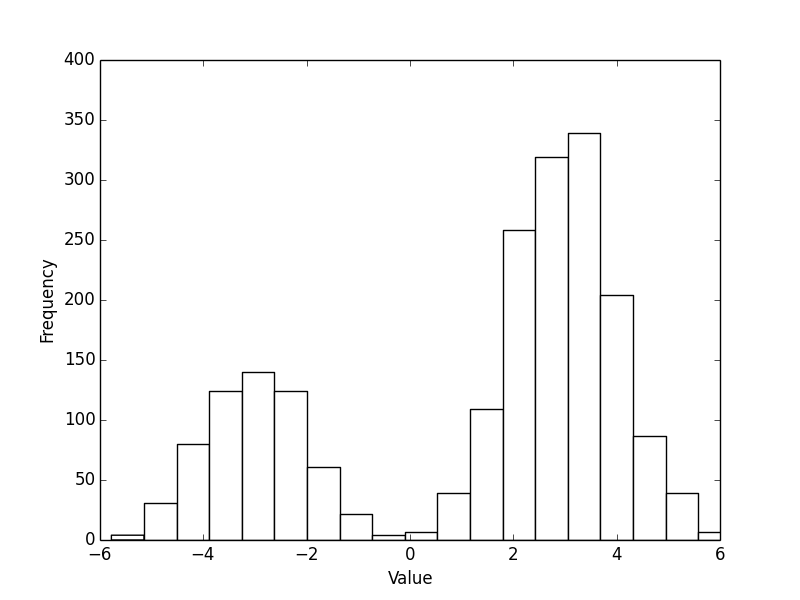
\includegraphics[width=218px]{graphs/hist.png}

The normalized log-likelihood of $X$ scored with model $\mathcal{F}$ and $\mathcal{G}$ equals

\begin{align*}
&\mathcal{F}_{score}\left(X\right) = \\
& \left(\sum\limits_{x \in X} \log \text{normPDF}\left(x, -3, 1\right)\right) / 2000 \approx -14 \\
&\mathcal{G}_{score}\left(X\right) = \\
&\left(\sum\limits_{x \in X} \log \text{normPDF}\left(x, 3, 1\right)\right) / 2000 \approx -7
\end{align*}

However, when you score the data with the interpolated model you get

\begin{align*}
&\sum\limits_{x \in X} \log \left( 0.3 \cdot \text{normPDF}\left(x, -3, 1\right) + 0.7 \cdot \text{normPDF}\left(x, 3, 1\right) \right) \\
&\approx -2
\end{align*}

which is significantly lower. Interpolating multiple N-gram models works in a similar manner to lower normalized log-likelihoods by better describing the generative story of the text.

\paragraph{Maximum Likelihood Estimator}

When a model is unsmoothed, it is the maximum likelihood estimator (MLE) as it will give the highest probability when run on the data the model was trained. For the full proof of this see Appendix B.

\subsubsection{Math}

\paragraph{NLP Distributions and Properties}

Language models have several constraints. The largest of these is that language must be valid probability distributions, with all probabilities between 0 and 1 and summing to 1.

\setcounter{equation}{0}

\begin{gather}
\forall w \in V : 0 \leq P\left(w\right) \leq 1 \\
\sum\limits_{w \in V} P\left(w\right) = 1
\end{gather}

Additionally, the marginal count will always equal the sum of the individual counts

$$ c\left(v\right) = \sum\limits_{w \in V} c\left(v, w\right) $$

\paragraph{Lagrange Multipliers}

The method of Lagrange multipliers is a way to find extrema of a function bounded by equality constraints. In formal terms the optimization problem is stated as
\begin{gather*}
\text{maximize } f\left(x\right) \\
\text{subject to } g\left(x\right) = c
\end{gather*}
One then uses the following equation
$$ \Lambda\left(x, \lambda \right) = f\left(x\right) + \lambda\left(g\left(x\right) - c \right) $$
and finds the derivative with respect to $x$ and $\lambda$. One can then set $\lambda$ to 0 to maximize the function.

One thing to note is that this find a point where the derivative is 0; this can be either a minima or maxima. 

Lagrange multipliers are central to the MLE proof in Appendix B, which acts as a good example of their use.

\paragraph{Entropy}
Entropy can be defined as a measure of the amount of information needed to represent a random variable on average. This can be calculated as follows
\begin{align*}
H\left(X\right) &= E\left[I\left(X\right)\right] \\
&= \sum\limits_i P\left(x=i\right) I\left(x=i\right) \\
&= - \sum\limits_i P\left(x=i\right) \log P\left(x=i\right)
\end{align*}

where $I\left(X\right)$ is the information content of $X$ and $E\left[X\right]$ is the expected value of random variable $X$.

A uniform probability distribution has the highest entropy, and a probability distribution with all of its mass on one event has the lowest (0).

\paragraph{Perplexity}

Perplexity is a measure of how well a probability model predicts a sample. It can be calculated as follows

$$ 2^{H\left(p\right)} = 2^{-\sum_x p\left(x\right) \log_2 p\left(x\right)}$$
% Is the sum over x normally N-grams in the held-out dataset?

\paragraph{KL Similarity}

KL Similarity is a measure of similarity between two probability models. It can calculated as follows

$$D_{KL}\left(P\|Q\right) = \sum\limits_i \ln\left(\frac{P\left(i\right)}{Q\left(i\right)}\right) P\left(i\right)$$

It is also a measure of information lost when $Q$ is used to approximate $P$. If $P$ and $Q$ are identical, then the KL similarity is equal to 0.

\paragraph{Cross Entropy}

Cross entropy is another method to estimate how well one probability distribution predicts another, similar to perplexity. It can be calculated as follows

\begin{align*}
H\left(p,q\right) &= E_p\left[-\log q\right] \\
&= -\sum_x p\left(x\right) \log q\left(x\right)
\end{align*}

\section{Methods \& Results}

\subsection{Python Implementation}

{\color{red} TwitterKov details}

\subsection{Performance Comparisons}

{\color{red} list vs dict vs trie}

\subsection{ACL 2014}

{\color{red} Summary of papers, new things I learned about}

\section{Summary}

\section{Acknowledgements}


%\begin{thebibliography}{}

%\end{thebibliography}

\appendix
\section{Additive Smoothing as a Linear Interpolation}

\begin{align}
P^*\left(w \vert v \right) &= \frac{c^*\left(v, w\right)}{\sum\limits_{w^` \in V} c^*\left(v, w \right)} \\
&= \frac{c \left( v, w \right) + \theta}{\sum\limits_{w^` \in V} \left( c\left( v, w \right) + \alpha \right)} \\
&= \frac{c \left( v, w \right) + \alpha}{c \left( v \right) + V\alpha} \\
&= \frac{c\left(v, w\right)}{c\left( v \right) + V\alpha} + \frac{\alpha}{c\left( v \right) + V\alpha} \\
&= \frac{c\left( v\right)}{c\left( v\right) + V\alpha} \frac{c\left(v, w\right)}{c\left( v \right)} + \frac{1}{V} \frac{V\alpha}{c\left( v \right) + V\alpha} \\
&= \frac{c\left( v\right)}{c\left( v\right) + V\alpha} \frac{c\left(v, w\right)}{c\left( v \right)} + \left( 1 - \frac{c\left( v\right)}{c\left( v\right) + V\alpha} \right) \frac{1}{V} \\
&= \lambda \frac{c\left(v, w\right)}{c\left( v \right)} + \left(1-\lambda\right) \frac{1}{V}
\end{align}

\section{Derivation of Maximum Likelihood Estimator}

Below I have shown the derivations for the Maximum Likelihood Estimators (MLEs) of both unigram and bigram models.

From the derivations below, it can be extrapolated that the MLE of an n-gram model would be

$$\phi_{t_1, t_2, \cdots , t_n} = \frac{c \left( t_1, t_2, \cdots , t_n \right)}{c \left( t_1, t_2, \cdots , t_{n - 1} \right)}$$

\subsection{Unigram}
Given $n$ tokens

$$ y_0, y_1, y_2, \cdots, y_n $$

With a vocabulary set 

$$ V = \left\{ v_0, v_1, v_2, \cdots v_m \right\} $$

Whose generative story is:

From probability vector $\theta$ draw

$$ y_i \: \lvert \: \theta \stackrel{i.i.d.}{\sim} \text{cat} \left( \theta \right) $$

The maximum likelihood estimator of $\theta$ is the probability distribution $\phi$ that maximizes the log-likelihood of observed data, calculated with

$$ L \left( \phi \right) = \sum \limits_{v \: \in \: V} c \left( v \right) \log{\phi_v} $$

To be derived is that the maximum likelihood estimator is

$$\phi_i = \frac{c \left( i \right)}{n}$$

To do this, you maximize the log-likelihood function, varying $\phi$ (restricted to valid probability distributions). This can be done with the method of Lagrange multipliers.

\begin{align*}
\max \limits_{\phi} \; L\left( \phi \right) \; \text{s.t.} \; \sum \limits_{v \in V} \phi_{v} = 1 \\
%
\Lambda \left( \phi, \lambda \right) = L\left( \phi \right) - \lambda \left( \sum \limits_{v \in V} \phi_{v} - 1 \right)
\end{align*}

The partial derivative of $\Lambda$ with respect to $\phi_i$ for any type $i$ is

\begin{align*}
%
\frac{\partial}{\partial \phi_i} \Lambda &= L^\prime \left( \phi \right) - \frac{\partial}{\partial \phi_i} \lambda \left( \sum \limits_{v \in V} \phi_{v} - 1 \right) \\
%
&= L^\prime \left( \phi \right) - \lambda \\
%
&= \frac{\partial}{\partial \phi_i} \left( \sum \limits_{v \in V} c \! \left( v \right) \log{\phi_v} \right) - \lambda \\
%
&= \frac{c \left( i \right)}{\phi_i} - \lambda
\end{align*}

This can be set to $0$ and be solved for $\phi_i$

\begin{align*}
\frac{c \left( i \right)}{\phi_i} - \lambda &= 0 \\
%
\frac{c \left( i \right)}{\phi_i} &= \lambda \\
%
\phi_{i} &= \frac{c \left( i \right)}{\lambda}
\end{align*}

The partial derivative of $\Lambda$ with respect to $\lambda$ is

\begin{align*}
\frac{\partial}{\partial \lambda} \Lambda = 1 - \sum \limits_{v \in V} \phi_{v}
\end{align*}

This can be set to $0$ and solved for $\lambda$, substituting $\phi_{v}$ for $ \frac{c \left( v \right)}{\lambda}$.

\begin{align*}
1 - \sum \limits_{v \in V} \phi_{v} &= 0 \\
%
1 - \sum \limits_{v \in V} \frac{c \left( v \right)}{\lambda} &= 0 \\
%
\sum \limits_{v \in V} \frac{c \left( v \right)}{\lambda} &= 1 \\
%
\lambda = \sum \limits_{v \in V} c \left( v \right) &= n
\end{align*}

It then becomes clear that the maximum likelihood estimator $\phi$ is

\begin{align*}
\phi_i &= \frac{c \left( i \right)}{n}
\end{align*}
%
%
%
\subsection{Bigram}

Given $n$ tokens

$$ y_0, y_1, y_2, \cdots, y_n $$

With a vocabulary set

$$ V = \left\{ v_0, v_1, v_2, \cdots, v_m \right\} $$

Whose generative story is:

From probability vector $\theta$ draw

$$ y_i \: \lvert \: y_{i - 1}, \theta \stackrel{i.i.d.}{\sim} \text{cat} \left( \theta_{i - 1} \right) $$

The maximum likelihood estimator of $\theta$ is the probability distribution $\phi$ that maximizes the log-likelihood of observed data, calculated with

$$ L \left( \phi \right) = \sum \limits_{v, w \in V} c \left( v, w \right) \log{\phi_{v, w}} $$

To be derived is that the maximum likelihood estimator is

$$\phi_{i, j} = \frac{c \left( i, j \right)}{ c \left( i \right)}$$

To do this, you maximize the log-likelihood function, varying $\phi$ (restricted to valid probability distributions). This can be done with the method of Lagrange multipliers.

\begin{align*}
&\max \limits_{\phi} \; L\left( \phi \right) \; \text{s.t.} \; \forall \; v \in V : \sum \limits_{w \in V} \phi_{v, w} = 1 \\
%
&\vec{\lambda} = \left( \lambda_1, \lambda_2, \cdots , \lambda_m \right) \notag \\
%
&\vec{G} = \left( \sum \limits_{w \in V} \phi_{v_1, w} - 1, \sum \limits_{w \in V} \phi_{v_2, w} - 1, \cdots , \sum \limits_{w \in V} \phi_{v_m, w} - 1 \right) \\
%
&\Lambda \left( \phi, \lambda \right) = L\left( \phi \right) - \vec{\lambda} \cdot \vec{G}
\end{align*}

The partial derivative of $\Lambda$ with respect to $\phi_{i, j}$ for any bigram $\left( i, j \right)$ is

\begin{align*}
%
\frac{\partial}{\partial \phi_{i, j}} \Lambda &= L^\prime \left( \phi \right) - \frac{\partial}{\partial \phi_{i, j}} \vec{\lambda} \cdot \vec{G} \\
%
&= L^\prime \left( \phi \right) - \lambda_i \\
%
&= \frac{\partial}{\partial \phi_{i, j}} \left( \sum \limits_{v, w \in V} c \! \left( v, w \right) \log{\phi_{v, w}} \right) - \lambda_i \\
%
&= \frac{c \left( i, j \right)}{\phi_{i, j}} - \lambda_i
\end{align*}

This can be set to $0$ and be solved for $\phi_{i, j}$

\begin{align*}
\frac{c \left( i, j \right)}{\phi_{i, j}} - \lambda_i &= 0 \\
%
\frac{c \left( i, j \right)}{\phi_{i, j}} &= \lambda_i \\
%
\phi_{i, j} &= \frac{c \left( i, j \right)}{\lambda_i}
\end{align*}

The partial derivative of $\Lambda$ with respect to $\lambda_i$ is

\begin{align*}
\frac{\partial}{\partial \lambda_i} \Lambda &= 1 - \sum \limits_{w \in V} \phi_{v_i, w}
\end{align*}

This can be set to $0$ and solved for $\lambda$, substituting $\phi_{v_i, w}$ for $ \frac{c \left( v_i, w \right)}{\lambda_i}$.

\begin{align*}
1 - \sum \limits_{w \in V} \phi_{v_i, w} &= 0 \\
%
1 - \sum \limits_{w \in V}  \frac{c \left( v_i, w \right)}{\lambda_i} &= 0 \\
%
\sum \limits_{w \in V}  \frac{c \left( v_i, w \right)}{\lambda_i} &= 1 \\
%
\lambda_i = \sum \limits_{w \in V} c \left( v_i, w \right) &= c \left( v_i \right)
\end{align*}

It then becomes clear that the maximum likelihood estimator $\phi$ is

\begin{align*}
\phi_{i, j} &= \frac{c \left( i, j \right)}{c \left( i \right)}
\end{align*}

\end{document}
